% Brief assessment of the RESONANCE AI4D Lab website.
% Build: lualatex assessment-brief.tex  (needs the IBM Plex Sans font installed)
\documentclass[10pt,a4paper]{article}

\usepackage[a4paper,top=15mm,bottom=17mm,left=16mm,right=16mm,footskip=8mm]{geometry}
\usepackage{fontspec}
\setmainfont{IBM Plex Sans}[
  BoldFont = IBM Plex Sans SemiBold,
  BoldItalicFont = IBM Plex Sans SemiBold Italic]
\newfontfamily\lightfont{IBM Plex Sans Light}
\usepackage{microtype}
\usepackage[table]{xcolor}
\usepackage{xltabular,booktabs,array,ragged2e}
\usepackage{tikz}
\usepackage[most]{tcolorbox}
\usepackage{enumitem}
\usepackage{fancyhdr}
\usepackage{lastpage}
\usepackage{graphicx}
\usepackage[hidelinks]{hyperref}

% ---- Palette ---------------------------------------------------------------
\definecolor{brand}{HTML}{005747}      % lab green, taken from the live site
\definecolor{brandtint}{HTML}{E8F1EF}
\definecolor{ink}{HTML}{1D2939}
\definecolor{muted}{HTML}{475467}
\definecolor{rule}{HTML}{D0D5DD}
\definecolor{critical}{HTML}{B42318}
\definecolor{high}{HTML}{C4320A}
\definecolor{medium}{HTML}{F5B000}
\definecolor{low}{HTML}{667085}

\color{ink}
\setlength{\parindent}{0pt}
\setlength{\parskip}{0pt}
\hyphenpenalty=10000\exhyphenpenalty=10000 % no word breaks in narrow columns
\hypersetup{colorlinks=true,urlcolor=brand,linkcolor=brand}

% ---- Severity tags ---------------------------------------------------------
\newcommand{\sevtag}[3]{\tikz[baseline=(t.base)]\node[fill=#1,text=#2,rounded corners=2.5pt,
  inner xsep=4pt,inner ysep=2.2pt,font=\scriptsize\bfseries,minimum width=15mm](t){#3};}
\newcommand{\critical}{\sevtag{critical}{white}{CRITICAL}}
\newcommand{\high}{\sevtag{high}{white}{HIGH}}
\newcommand{\medium}{\sevtag{medium}{ink}{MEDIUM}}
\newcommand{\low}{\sevtag{low}{white}{LOW}}

% ---- Issue row: number, name, evidence, severity, recommendation ----------
\newcommand{\issue}[5]{%
  \leavevmode{\color{muted}\footnotesize #1} &
  \textbf{#2}\newline{\color{muted}\footnotesize #3} &
  #4 &
  {\footnotesize #5}\\\arrayrulecolor{rule}\midrule}

% ---- Headline numbers ------------------------------------------------------
\newtcolorbox{metric}{enhanced,colback=brandtint,colframe=brandtint,arc=3pt,
  boxrule=0pt,left=7pt,right=6pt,top=5pt,bottom=5pt,equal height group=metrics}
\newcommand{\metricbox}[2]{%
  \begin{metric}{\fontsize{19}{21}\selectfont\bfseries\color{brand}#1}\par
  \vspace{2pt}{\RaggedRight\footnotesize\color{muted}#2\par}\end{metric}}

% ---- Page style ------------------------------------------------------------
\pagestyle{fancy}\fancyhf{}
\renewcommand{\headrulewidth}{0pt}
\fancyfoot[L]{\scriptsize\color{muted}RESONANCE AI4D Lab website: brief assessment}
\fancyfoot[R]{\scriptsize\color{muted}\thepage\,/\,\pageref{LastPage}}

\newcommand{\sectionhead}[1]{\vspace{11pt}{\small\bfseries\color{brand}\MakeUppercase{#1}}\par\vspace{3pt}}
\setlength{\LTpre}{0pt}\setlength{\LTpost}{4pt}

\begin{document}

% ---- Title -----------------------------------------------------------------
{\footnotesize\bfseries\color{brand}BRIEF ASSESSMENT\quad\mdseries\color{muted}\lightfont October 2026}\par
\vspace{3pt}
{\fontsize{22}{26}\selectfont\bfseries RESONANCE AI4D Lab website}\par
\vspace{4pt}
{\small\color{muted}Site reviewed: \href{https://sites.google.com/aait.edu.et/resonance-lab/home}{sites.google.com/aait.edu.et/resonance-lab} (all 9 pages), 3--4 October 2026\\
Method: Chrome at 1440\,px and 390\,px, Lighthouse 12, manual accessibility review, comparison with four similar sites}\par
\vspace{8pt}
{\color{brand}\rule{\linewidth}{1.4pt}}\par
\vspace{9pt}

% ---- Summary ---------------------------------------------------------------
{\small
The lab's content is strong: a clear mission, four well-defined research themes and a detailed call for
applications. \textbf{The way the site is built hides most of it.} Every section is a Google Sites
\emph{Custom embed}, a separate document inside an iframe. Phones cut these off, search can't read them,
and each one loads its own copy of a development-only CSS framework. Outdated dates, placeholder text and
an inconsistent visual style then undercut the credibility a university lab needs.\par}

\vspace{9pt}
\begin{tcbraster}[raster columns=4,raster column skip=3.5mm,raster equal height]
  \metricbox{34\,/\,100}{Lighthouse performance score on mobile}
  \metricbox{27.3\,s}{until the main content appears on a phone}
  \metricbox{5.6\,MB}{downloaded for the homepage, in 65 requests}
  \metricbox{0}{site-search results for ``agriculture'', a core research theme}
\end{tcbraster}

% ---- Issues ----------------------------------------------------------------
\sectionhead{Issues and recommendations, most critical first}

{\renewcommand{\arraystretch}{1.25}
\begin{xltabular}{\linewidth}{@{}>{\RaggedLeft}p{4mm}>{\RaggedRight}X>{\centering\arraybackslash}p{17mm}>{\RaggedRight}p{60mm}@{}}
{\scriptsize\color{muted}\#} & {\scriptsize\bfseries\color{muted}ISSUE} & {\scriptsize\bfseries\color{muted}SEVERITY} & {\scriptsize\bfseries\color{muted}RECOMMENDATION}\\
\arrayrulecolor{ink}\midrule
\endhead

\issue{1}{Content cut off on phones}
  {Each section is an iframe with a fixed height ratio. At 390\,px the homepage shows only section headings, and the Team page shows no names.}
  {\critical}
  {Move content out of Custom embeds into real page content (native Google Sites blocks or a small static site).}

\issue{2}{Outdated and placeholder content}
  {The homepage says applications ``are now open'' for a call that closed in August 2025. Publications lists ``Title goes here''; the phone number is ``+251 XXX XXX XXXX''.}
  {\critical}
  {Mark the 2025/26 call as closed, remove placeholders until real entries exist, and give News \& Events an owner and a review date.}

\issue{3}{Very slow to load}
  {A 1.1\,MB seal is shown at 56\,px, a 1.7\,MB PNG draws a simple gradient, and each embed loads Tailwind's development CDN.}
  {\critical}
  {Draw the hero background in CSS, resize the seal to about 10\,KB, and drop the per-embed CDN and fonts.}

\issue{4}{Homepage doesn't say who the lab is}
  {RESONANCE is never spelled out; Addis Ababa University appears only as a seal. The first screen holds only the name, with no mission or contact details.}
  {\high}
  {Open with the full name, a one-line mission and the AAU\,/\,CTBE affiliation.}

\issue{5}{Navigation hidden and inconsistent}
  {All pages are nested under a ``Home'' dropdown. Boxy button rows change on every page, labels vary, and Contact is missing from all of them.}
  {\high}
  {One flat text menu with consistent labels, the current page marked, and a proper menu on phones.}

\issue{6}{Invisible to search}
  {Site search finds nothing, because the text lives inside embeds. Page descriptions read ``Our Partners:'', ``About'', ``Team''.}
  {\high}
  {Real page content, with a descriptive title and description for every page.}

\issue{7}{Accessibility barriers}
  {Logos have no alt text, and the white-on-lime banner has 2.05\,:\,1 contrast. Emoji are read aloud, and every iframe is announced as ``Custom embed''.}
  {\high}
  {Add alt text, meet WCAG AA contrast, use one heading outline, and add visible focus states and a skip link.}

\issue{8}{Emoji used as icons}
  {They look different on every device and read as informal next to a university seal.}
  {\medium}
  {Simple SVG line icons in the brand colour.}

\issue{9}{Inconsistent typography}
  {Five font families on one page: Roboto, Google Sans, Playfair Display, Open Sans and Inter.}
  {\medium}
  {Two typefaces: the lab's own Playfair Display for headings and Inter for text.}

\issue{10}{Off-brand colours, boxy layout}
  {Tailwind blue and a lime gradient next to the lab green; the theme colour-coding is saturated and never explained; cards are nested inside grey panels.}
  {\medium}
  {The brand green (\#005747) plus the theme colours tuned for contrast, and one card style.}

\issue{11}{Header title too long}
  {``RESONANCE AI4D Lab @CTBE'' in a display serif reads like a social-media handle, and the emblem is the AAU seal, not a lab mark.}
  {\medium}
  {A short wordmark, with ``AI4D Lab · Addis Ababa University'' set small beneath it.}

\issue{12}{Oversized, unbalanced footer}
  {Partner logos run full width at uneven sizes (about 600\,px tall on phones), with no alt text and no address, email or links.}
  {\medium}
  {A compact footer: contact details, page links, and partner logos at equal height.}

\issue{13}{Placeholder team avatars}
  {Coloured circles with first names written inside (``Dr.\ Elefelious'' shrunk to fit), plus six ``To be recruited'' cards.}
  {\medium}
  {Real photos (with consent) or two-letter initials in each person's theme colour, and open roles listed in one line.}

\issue{14}{Inconsistent naming and copy}
  {``Resonance Lab'', ``RESONANCE AI4D Lab'' and ``Resonance AI4D Lab'' all appear. There are small errors (``an Masters position''), and the Masters entry requirement differs between pages.}
  {\low}
  {One copy-editing pass and one official name.}
\end{xltabular}}


% ---- Evidence strip --------------------------------------------------------
\sectionhead{Evidence from the live site}
\newcommand{\shot}[3]{\begin{minipage}[t]{#1}\setlength{\fboxsep}{0pt}\setlength{\fboxrule}{0.4pt}%
  {\color{rule}\fbox{#2}}\par\vspace{2pt}{\RaggedRight\scriptsize\color{muted}#3\par}\end{minipage}}
\noindent
\shot{45mm}{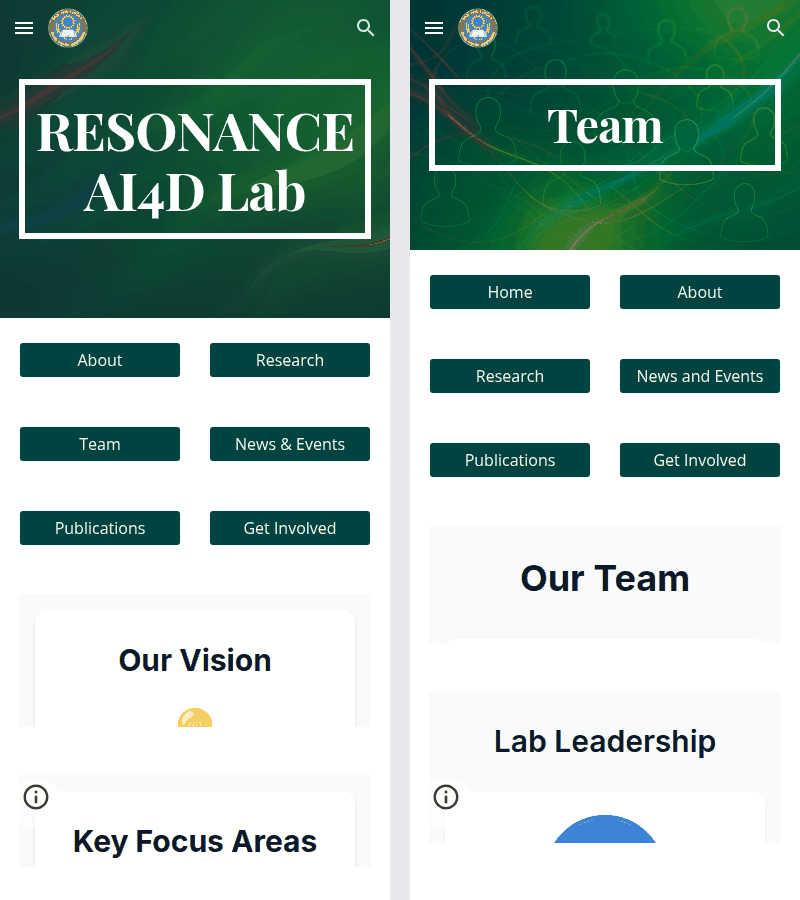
\includegraphics[height=33mm,trim=0 0 0 300,clip]{../assessment/01-mobile-clipping.png}}{Issue 1: Home and Team at phone width}\hfill
\shot{44.5mm}{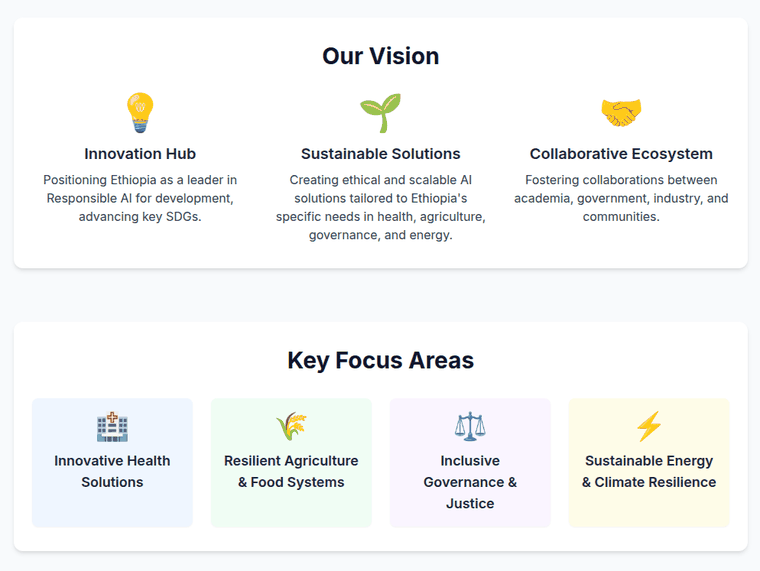
\includegraphics[height=33mm]{../assessment/03-emoji-icons.png}}{Issue 8: emoji used as icons}\hfill
\shot{81mm}{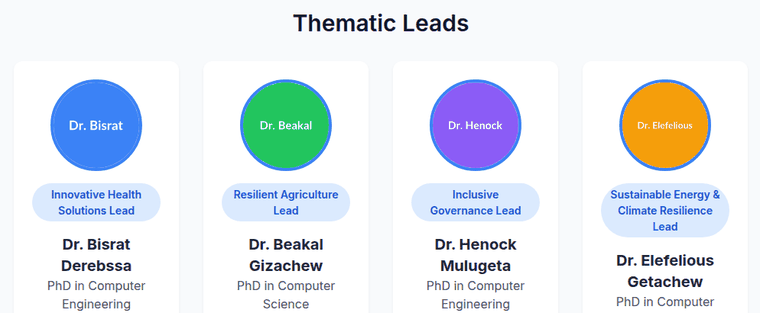
\includegraphics[height=33mm]{../assessment/04-team-avatars.png}}{Issue 13: placeholder avatars with names inside}\par
\vspace{6pt}\noindent
\shot{82.5mm}{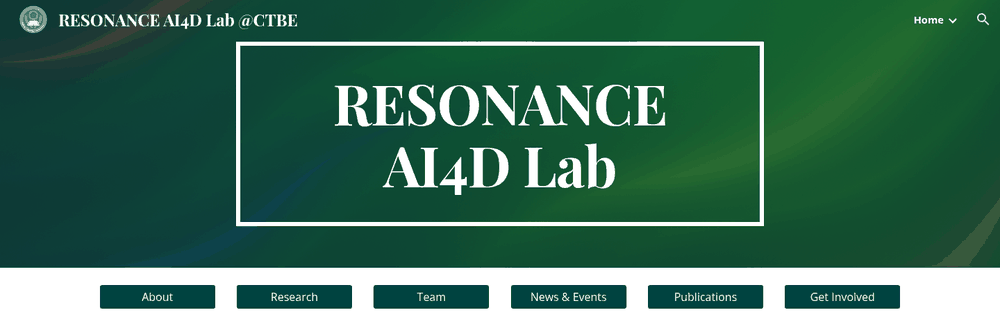
\includegraphics[height=26.5mm]{../assessment/02-header-hero-nav.png}}{Issues 5 and 11: long title, empty hero, boxy button row}\hfill
\shot{90.5mm}{
\includegraphics[height=26.5mm]{../assessment/07-footer-partners.png}}{Issue 12: oversized partner logos; no contact details}\par
\vspace{4pt}

% ---- Closing panels --------------------------------------------------------
\vspace{2pt}
\begin{tcbraster}[raster columns=2,raster column skip=4mm,raster equal height]
\begin{tcolorbox}[enhanced,colback=white,colframe=rule,boxrule=0.5pt,arc=3pt,left=8pt,right=8pt,top=7pt,bottom=7pt]
{\scriptsize\bfseries\color{brand}PATTERNS FROM COMPARABLE SITES}\par\vspace{4pt}
{\footnotesize\color{muted}Makerere AI Lab, Stanford HAI, Masakhane and AI4D Africa}\par\vspace{4pt}
\begin{itemize}[leftmargin=10pt,itemsep=1pt,topsep=0pt,label={\color{brand}\textbullet}]\footnotesize
  \item One line on the first screen saying who they are and where
  \item A single row of text links for navigation
  \item SVG icons, and one or two typefaces
  \item A compact footer with contact details and logos at equal height
  \item Masakhane also runs on Google Sites but keeps text in the page, so it reads fine on phones
\end{itemize}
\end{tcolorbox}
\begin{tcolorbox}[enhanced,colback=brandtint,colframe=brandtint,boxrule=0pt,arc=3pt,left=8pt,right=8pt,top=7pt,bottom=7pt]
{\scriptsize\bfseries\color{brand}WHAT THE HOMEPAGE PROTOTYPE COVERS}\par\vspace{4pt}
{\footnotesize Issues 1 and 3--12 on the homepage, plus its parts of 2 (call status shown from its dates, no
placeholders), 13 (initials) and 14 (one name). All content comes from the live site; nothing is invented.}\par\vspace{5pt}
{\scriptsize\bfseries\color{brand}NEEDS THE LAB}\par\vspace{3pt}
{\footnotesize A real publications list, the phone number, team photos, keeping News \& Events up to date, and a lab logo.}
\end{tcolorbox}
\end{tcbraster}

\vspace{6pt}
{\scriptsize\color{muted}Full assessment with screenshots, measurements and benchmark comparison: \textbf{ASSESSMENT.md} in the project repository.}

\end{document}
